\subsection{How many references should train the auditor?}
An exploratory extension fixes the total cost at 280 references per 1,000-record
sample. It uses the same five formula folds but draws nested random prefixes of
10, 20, 50 or 100 records from each designated seed fold, alongside the full fold
(mean size 200). Five deterministic permutations are used per fold. The remaining
four folds form a fixed audit pool, independent of prefix size. Unused seed-fold
records are excluded from this pool. All seeds contain at least three formulas;
the original grouped penalty selection and tree settings are retained.

A learned policy uses $m$ references for training and $280-m$ for acquisitions.
Direct policies spend all 280 on the same pool. Only pool discoveries count,
with positives defined as the worst $\lceil0.1|\mathcal U|\rceil$ pool records.
This transfer-to-unseen-formulas endpoint intentionally differs from the earlier
whole-sample recall, which credited seed discoveries. Repeats are averaged within
fold before summarizing the five overlapping scenarios; they are not independent
confirmation datasets. The extension protocol was recorded after examining the
primary results, and no fresh data were introduced.

\begin{figure}[t]
\centering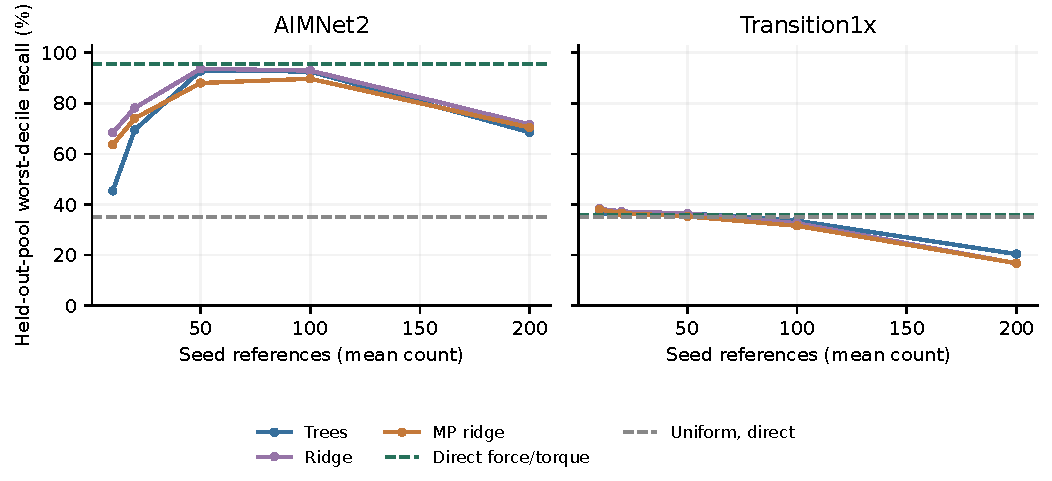
\includegraphics[width=\linewidth]{figures/small_seed_budget.pdf}
\caption{Reference allocation at a fixed total budget of 280. Increasing seed
count leaves fewer acquisitions in the fixed held-out pool. Points average five
seed permutations within each of five formula scenarios. The full-fold point
has mean size 200; its actual size varies by scenario. Direct-policy lines use
280 pool acquisitions throughout.}
\label{fig:smallseed}
\end{figure}

With 50 seed references, log-error trees recover 92.8\%
of the pool's worst decile on AIMNet2 and 36.5\% on
Transition1x. Using the entire seed fold gives 68.5\% and
20.4\%, respectively (Figure~\ref{fig:smallseed}).
At 50 references, ordinary ridge gives 93.7\% and
36.5\%, while MP-pooled ridge gives
88.0\% and 35.3\%.
Direct force/torque screening gives 95.5\% and
36.1\% on these pools.

These curves measure the combined effects of predictor quality and reference
allocation, not prediction error at equal acquisition counts. More training
references need not produce more discoveries under a fixed total budget. The
comparison does not establish a universal optimal seed size, an RMT advantage,
or transfer from these molecular samples to a substantially larger database.
